\documentclass[10pt]{article}
\usepackage[polish]{babel}
\usepackage[utf8]{inputenc}
\usepackage[T1]{fontenc}
\usepackage{graphicx}
\usepackage[export]{adjustbox}
\graphicspath{ {./images/} }
\usepackage{amsmath}
\usepackage{amsfonts}
\usepackage{amssymb}
\usepackage[version=4]{mhchem}
\usepackage{stmaryrd}
\usepackage{multirow}

\title{EGZAMIN MATURALNY Z MATEMATYKI }

\author{}
\date{}


\begin{document}
\maketitle
\begin{center}
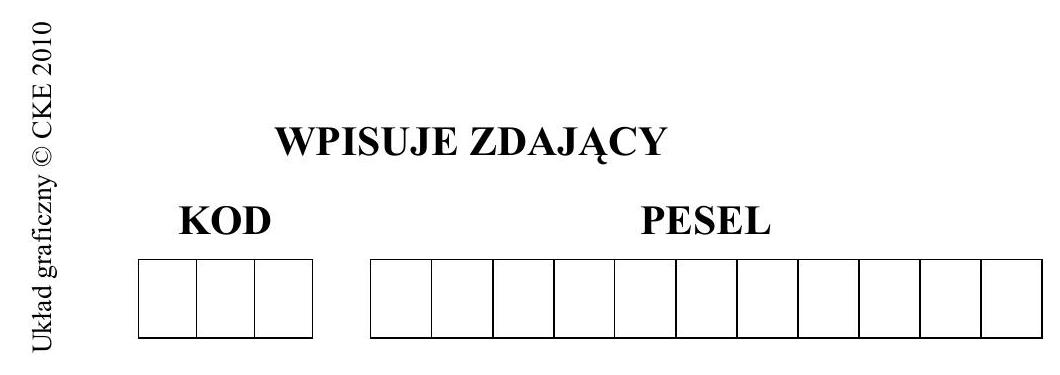
\includegraphics[max width=\textwidth]{2024_11_21_5b6b7ffa9006e3f448adg-01(1)}
\end{center}

\begin{center}
\begin{tabular}{c|}
\hline
Miejsce \\
na naklejke \\
z kodem \\
 \\
\hline
\end{tabular}
\end{center}

POZIOM PODSTAWOWY

\begin{enumerate}
  \item Sprawdź, czy arkusz egzaminacyjny zawiera 20 stron (zadania 1-33). Ewentualny brak zgłoś przewodniczącemu zespołu nadzorującego egzamin.
  \item Rozwiazzania zadań i odpowiedzi wpisuj w miejscu na to przeznaczonym.
  \item Odpowiedzi do zadań zamkniętych (1-23) przenieś na kartę odpowiedzi, zaznaczając je w części karty przeznaczonej dla zdającego. Zamaluj \(\square\) pola do tego przeznaczone. Błędne zaznaczenie otocz kółkiem i zaznacz właściwe.
  \item Pamiętaj, że pominięcie argumentacji lub istotnych obliczeń w rozwiązaniu zadania otwartego (24-33) może
\end{enumerate}

Czas pracy: 170 minut\\
spowodować, że za to rozwiązanie nie będziesz mógł dostać pełnej liczby punktów.\\
5. Pisz czytelnie i używaj tylko długopisu lub pióra z czarnym tuszem lub atramentem.\\
6. Nie używaj korektora, a błędne zapisy wyraźnie przekreśl.\\
7. Pamiętaj, że zapisy w brudnopisie nie będą oceniane.\\
8. Możesz korzystać z zestawu wzorów matematycznych, cyrkla i linijki oraz kalkulatora.\\
9. Na karcie odpowiedzi wpisz swój numer PESEL i przyklej naklejkę z kodem.\\
10. Nie wpisuj żadnych znaków w części przeznaczonej dla egzaminatora.

\section*{Liczba punktów}
do uzyskania: 50\\

\includegraphics[max width=\textwidth, center]{2024_11_21_5b6b7ffa9006e3f448adg-01}

MMA-P1\_1P-112

\section*{ZADANIA ZAMKNIĘTE}
W zadaniach od 1. do 23. wybierz izaznacz na karcie odpowiedzi poprawna odpowiedź.

\section*{Zadanie 1. (1 pkt)}
Wskaż nierówność, którą spełnia liczba \(\pi\).\\
A. \(|x+1|>5\)\\
B. \(|x-1|<2\)\\
C. \(\left|x+\frac{2}{3}\right| \leq 4\)\\
D. \(\left|x-\frac{1}{3}\right| \geq 3\)

\section*{Zadanie 2. (1 pkt)}
Pierwsza rata, która stanowi \(9 \%\) ceny roweru, jest równa 189 zł. Rower kosztuje\\
A. 1701 zt .\\
B. 2100 zt .\\
C. 1890 zt .\\
D. \(2091 \mathrm{zł}\).

\section*{Zadanie 3. (1 pkt)}
Wyrażenie \(5 a^{2}-10 a b+15 a\) jest równe iloczynowi\\
A. \(5 a^{2}(1-10 b+3)\)\\
B. \(5 a(a-2 b+3)\)\\
C. \(5 a(a-10 b+15)\)\\
D. \(5(a-2 b+3)\)

\section*{Zadanie 4. (1 pkt)}
Układ równań \(\left\{\begin{array}{l}4 x+2 y=10 \\ 6 x+a y=15\end{array}\right.\) ma nieskończenie wiele rozwiązań, jeśli\\
A. \(a=-1\)\\
B. \(a=0\)\\
C. \(a=2\)\\
D. \(a=3\)

\section*{Zadanie 5. (1 pkt)}
Rozwiązanie równania \(x(x+3)-49=x(x-4)\) należy do przedziału\\
A. \((-\infty, 3)\)\\
B. \((10,+\infty)\)\\
C. \((-5,-1)\)\\
D. \((2,+\infty)\)

\section*{Zadanie 6. (1 pkt)}
Najmniejszą liczbą całkowitą należącą do zbioru rozwiązań nierówności \(\frac{3}{8}+\frac{x}{6}<\frac{5 x}{12}\) jest\\
A. 1\\
B. 2\\
C. -1\\
D. -2

\section*{Zadanie 7. (1 pkt)}
Wskaż, który zbiór przedstawiony na osi liczbowej jest zbiorem liczb spełniających jednocześnie następujące nierówności: \(3(x-1)(x-5) \leq 0\) i \(x>1\).\\
A.\\
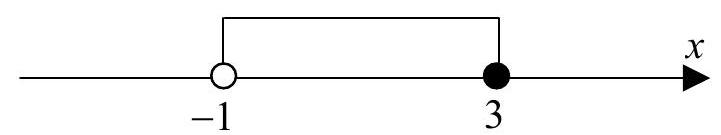
\includegraphics[max width=\textwidth, center]{2024_11_21_5b6b7ffa9006e3f448adg-02(1)}\\
B.\\
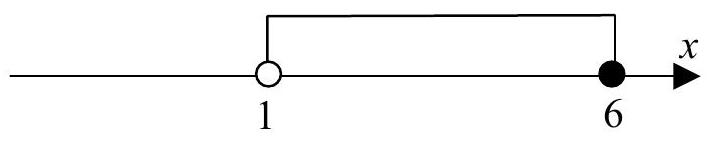
\includegraphics[max width=\textwidth, center]{2024_11_21_5b6b7ffa9006e3f448adg-02(3)}\\
C.\\
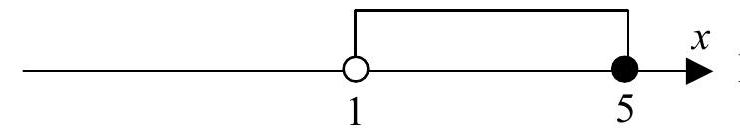
\includegraphics[max width=\textwidth, center]{2024_11_21_5b6b7ffa9006e3f448adg-02(2)}\\
D.\\
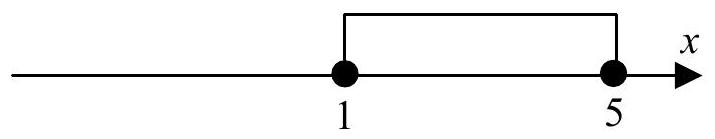
\includegraphics[max width=\textwidth, center]{2024_11_21_5b6b7ffa9006e3f448adg-02}

\section*{BRUDNOPIS}
\begin{center}

\includegraphics[max width=\textwidth]{2024_11_21_5b6b7ffa9006e3f448adg-03}
\end{center}

\section*{Zadanie 8. (1 pkt)}
Wyrażenie \(\log _{4}(2 x-1)\) jest określone dla wszystkich liczb \(x\) spełniajacych warunek\\
A. \(x \leq \frac{1}{2}\)\\
B. \(x>\frac{1}{2}\)\\
C. \(x \leq 0\)\\
D. \(x>0\)

\section*{Zadanie 9. (1 pkt)}
Dane są funkcje liniowe \(f(x)=x-2\) oraz \(g(x)=x+4\) określone dla wszystkich liczb rzeczywistych \(x\). Wskaż, który z poniższych wykresów jest wykresem funkcji \(h(x)=f(x) \cdot g(x)\).\\
A.\\
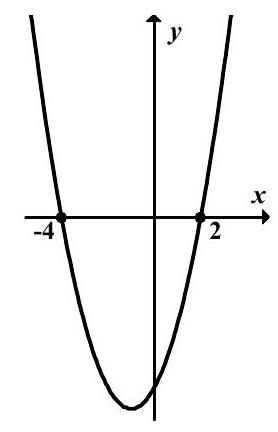
\includegraphics[max width=\textwidth, center]{2024_11_21_5b6b7ffa9006e3f448adg-04}\\
B.\\
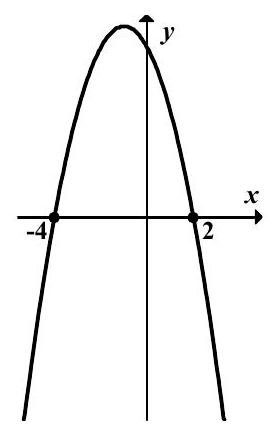
\includegraphics[max width=\textwidth, center]{2024_11_21_5b6b7ffa9006e3f448adg-04(3)}\\
C.\\
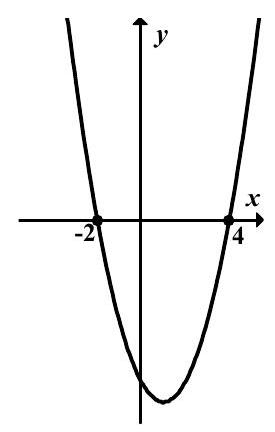
\includegraphics[max width=\textwidth, center]{2024_11_21_5b6b7ffa9006e3f448adg-04(2)}\\
D.\\
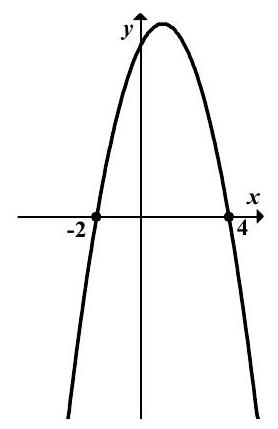
\includegraphics[max width=\textwidth, center]{2024_11_21_5b6b7ffa9006e3f448adg-04(1)}

\section*{Zadanie 10 (1 pkt)}
Funkcja liniowa określona jest wzorem \(f(x)=-\sqrt{2} x+4\). Miejscem zerowym tej funkcji jest liczba\\
A. \(-2 \sqrt{2}\)\\
B. \(\frac{\sqrt{2}}{2}\)\\
C. \(-\frac{\sqrt{2}}{2}\)\\
D. \(2 \sqrt{2}\)

\section*{Zadanie 11. (1 pkt)}
Dany jest nieskończony ciagg geometryczny \(\left(a_{n}\right)\), w którym \(a_{3}=1\) i \(a_{4}=\frac{2}{3}\). Wtedy\\
A. \(a_{1}=\frac{2}{3}\)\\
B. \(a_{1}=\frac{4}{9}\)\\
C. \(a_{1}=\frac{3}{2}\)\\
D. \(a_{1}=\frac{9}{4}\)

\section*{Zadanie 12. (1 pkt)}
Dany jest nieskończony rosnący ciag arytmetyczny \(\left(a_{n}\right)\) o wyrazach dodatnich. Wtedy\\
A. \(a_{4}+a_{7}=a_{10}\)\\
B. \(a_{4}+a_{6}=a_{3}+a_{8}\)\\
C. \(a_{2}+a_{9}=a_{3}+a_{8}\)\\
D. \(a_{5}+a_{7}=2 a_{8}\)

\section*{Zadanie 13. (1 pkt)}
Kąt \(\alpha\) jest ostry i \(\cos \alpha=\frac{5}{13}\). Wtedy\\
A. \(\sin \alpha=\frac{12}{13}\) oraz \(\operatorname{tg} \alpha=\frac{12}{5}\)\\
B. \(\sin \alpha=\frac{12}{13}\) oraz \(\operatorname{tg} \alpha=\frac{5}{12}\)\\
C. \(\sin \alpha=\frac{12}{5}\) oraz \(\operatorname{tg} \alpha=\frac{12}{13}\)\\
D. \(\sin \alpha=\frac{5}{12}\) oraz \(\operatorname{tg} \alpha=\frac{12}{13}\)

\section*{BRUDNOPIS}
\begin{center}

\includegraphics[max width=\textwidth]{2024_11_21_5b6b7ffa9006e3f448adg-05}
\end{center}

\section*{Zadanie 14. (1 pkt)}
Wartość wyrażenia \(\frac{\sin ^{2} 38^{\circ}+\cos ^{2} 38^{\circ}-1}{\sin ^{2} 52^{\circ}+\cos ^{2} 52^{\circ}+1}\) jest równa\\
A. \(\frac{1}{2}\)\\
B. 0\\
C. \(-\frac{1}{2}\)\\
D. 1

\section*{Zadanie 15. (1 pkt)}
W prostopadłościanie \(A B C D E F G H\) mamy: \(|A B|=5,|A D|=4,|A E|=3\). Który z odcinków \(A B, B G, G E, E B\) jest najdłuższy?\\
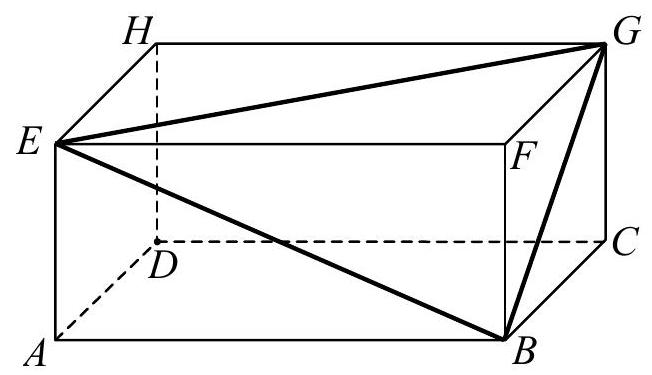
\includegraphics[max width=\textwidth, center]{2024_11_21_5b6b7ffa9006e3f448adg-06(1)}\\
A. \(A B\)\\
B. \(B G\)\\
C. \(G E\)\\
D. \(E B\)

\section*{Zadanie 16. (1 pkt)}
Punkt \(O\) jest środkiem okręgu. Kąt wpisany \(\alpha\) ma miarę\\
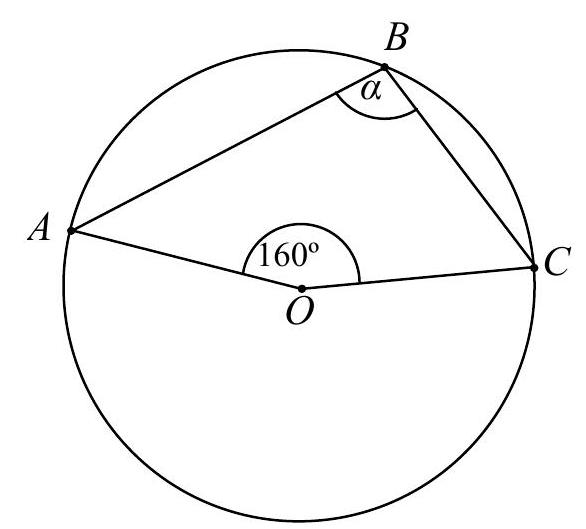
\includegraphics[max width=\textwidth, center]{2024_11_21_5b6b7ffa9006e3f448adg-06}\\
A. \(80^{\circ}\)\\
B. \(100^{\circ}\)\\
C. \(110^{\circ}\)\\
D. \(120^{\circ}\)

\section*{Zadanie 17. (1 pkt)}
Wysokość rombu o boku długości 6 i kącie ostrym \(60^{\circ}\) jest równa\\
A. \(3 \sqrt{3}\)\\
B. 3\\
C. \(6 \sqrt{3}\)\\
D. 6

\section*{Zadanie 18. (1 pkt)}
Prosta \(k\) ma równanie \(y=2 x-3\). Wskaż równanie prostej \(l\) równoległej do prostej \(k\) i przechodzącej przez punkt \(D\) o wspórzzędnych \((-2,1)\).\\
A. \(y=-2 x+3\)\\
B. \(y=2 x+1\)\\
C. \(y=2 x+5\)\\
D. \(y=-x+1\)

\section*{BRUDNOPIS}
\begin{center}

\includegraphics[max width=\textwidth]{2024_11_21_5b6b7ffa9006e3f448adg-07}
\end{center}

Zadanie 19. (1 pkt)\\
Styczną do okręgu \((x-1)^{2}+y^{2}-4=0\) jest prosta o równaniu\\
A. \(x=1\)\\
B. \(x=3\)\\
C. \(y=0\)\\
D. \(y=4\)

\section*{Zadanie 20. (1 pkt)}
Pole powierzchni całkowitej sześcianu jest równe 54. Długość przekątnej tego sześcianu jest równa\\
A. \(\sqrt{6}\)\\
B. 3\\
C. 9\\
D. \(3 \sqrt{3}\)

\section*{Zadanie 21. (1 pkt)}
Objętość stożka o wysokości 8 i średnicy podstawy 12 jest równa\\
A. \(124 \pi\)\\
B. \(96 \pi\)\\
C. \(64 \pi\)\\
D. \(32 \pi\)

\section*{Zadanie 22. (1 pkt)}
Rzucamy dwa razy symetryczną sześcienną kostką do gry. Prawdopodobieństwo otrzymania sumy oczek równej trzy wynosi\\
A. \(\frac{1}{6}\)\\
B. \(\frac{1}{9}\)\\
C. \(\frac{1}{12}\)\\
D. \(\frac{1}{18}\)

\section*{Zadanie 23. (1 pkt)}
Uczniowie pewnej klasy zostali poproszeni o odpowiedź na pytanie: „Ile osób liczy twoja rodzina?" Wyniki przedstawiono w tabeli:

\begin{center}
\begin{tabular}{|c|c|}
\hline
\begin{tabular}{c}
Liczba osób \\
w rodzinie \\
\end{tabular} & \begin{tabular}{c}
liczba \\
uczniów \\
\end{tabular} \\
\hline
3 & 6 \\
\hline
4 & 12 \\
\hline
\(x\) & 2 \\
\hline
\end{tabular}
\end{center}

Średnia liczba osób w rodzinie dla uczniów tej klasy jest równa 4. Wtedy liczba \(x\) jest równa\\
A. 3\\
B. 4\\
C. 5\\
D. 7

\section*{BRUDNOPIS}
\begin{center}

\includegraphics[max width=\textwidth]{2024_11_21_5b6b7ffa9006e3f448adg-09}
\end{center}

\section*{ZADANIA OTWARTE}
\section*{Rozwiazania zadań o numerach od 24. do 33. należ̀y zapisać w wyznaczonych miejscach pod treściq zadania.}
\section*{Zadanie 24. (2 pkt)}
Rozwiąż nierówność \(3 x^{2}-10 x+3 \leq 0\).\\

\includegraphics[max width=\textwidth, center]{2024_11_21_5b6b7ffa9006e3f448adg-10(1)}

Odpowiedź:

\section*{Zadanie 25. (2 pkt)}
Uzasadnij, że jeżeli \(a+b=1\) i \(a^{2}+b^{2}=7\), to \(a^{4}+b^{4}=31\).\\

\includegraphics[max width=\textwidth, center]{2024_11_21_5b6b7ffa9006e3f448adg-10}

\section*{Zadanie 26. (2 pkt)}
Na rysunku przedstawiono wykres funkcji \(f\).\\
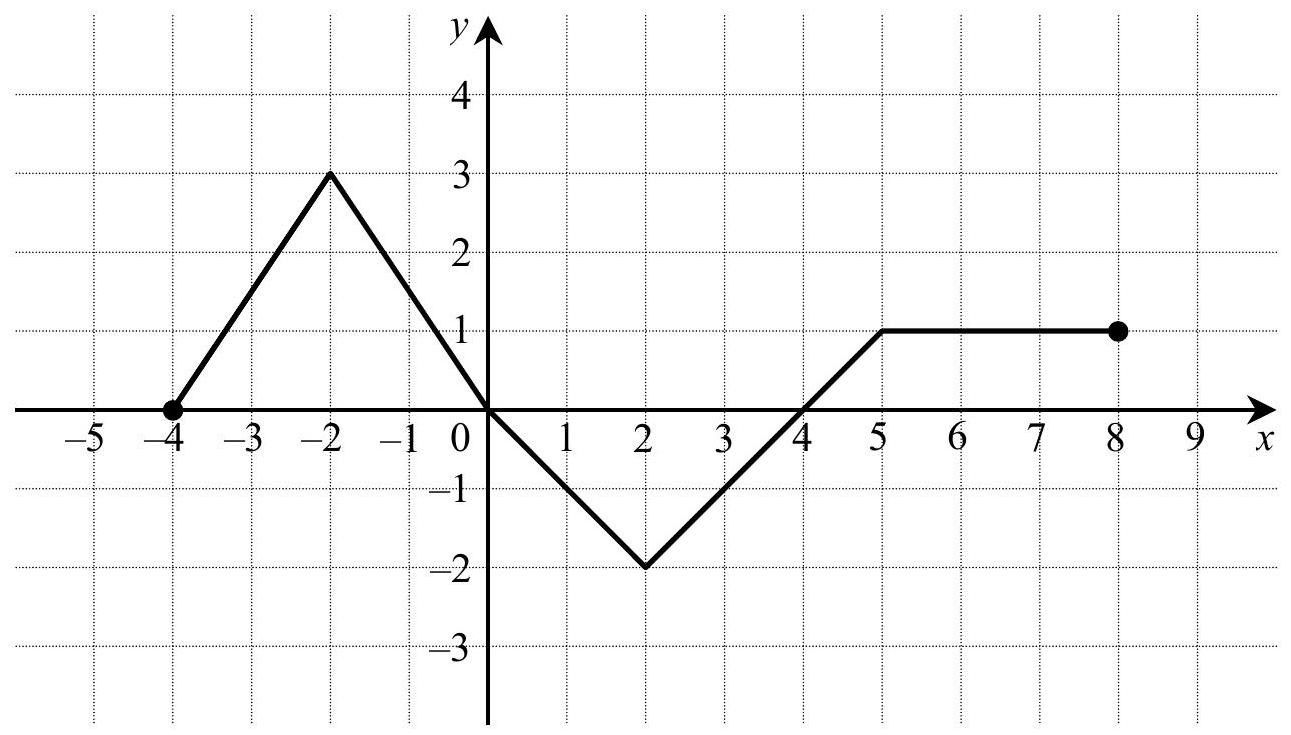
\includegraphics[max width=\textwidth, center]{2024_11_21_5b6b7ffa9006e3f448adg-11}

Odczytaj z wykresu i zapisz:\\
a) zbiór wartości funkcji \(f\),\\
b) przedział maksymalnej długości, w którym funkcja \(f\) jest malejąca.\\

\includegraphics[max width=\textwidth, center]{2024_11_21_5b6b7ffa9006e3f448adg-11(1)}

Odpowiedź:

\begin{center}
\begin{tabular}{|c|l|c|c|c|}
\hline
\multirow{2}{*}{\begin{tabular}{c}
Wypetnia \\
egzaminator \\
\end{tabular}} & Nr zadania & 24. & 25. & 26. \\
\cline { 2 - 5 }
 & Maks. liczba pkt & 2 & 2 & 2 \\
\cline { 2 - 5 }
 & Uzyskana liczba pkt &  &  &  \\
\hline
\end{tabular}
\end{center}

\section*{Zadanie 27. (2 pkt)}
Liczby \(x, y, 19 \mathrm{w}\) podanej kolejności tworzą ciąg arytmetyczny, przy czym \(x+y=8\). Oblicz \(x\) i \(y\).

\begin{center}
\begin{tabular}{|c|c|c|c|c|c|c|c|c|c|c|c|c|c|c|c|c|c|c|c|c|c|}
\hline
- &  &  &  &  &  &  &  &  &  &  &  &  &  &  &  &  &  &  &  &  &  \\
\hline
- &  &  &  &  &  &  &  &  &  &  &  &  &  &  &  &  &  &  &  &  &  \\
\hline
- &  &  &  &  &  &  &  &  &  &  &  &  &  &  &  &  &  &  &  &  &  \\
\hline
- &  &  &  &  &  &  &  &  &  &  &  &  &  &  &  &  &  &  &  &  &  \\
\hline
 &  &  &  &  &  &  &  &  &  &  &  &  &  &  &  &  &  &  &  &  &  \\
\hline
- &  &  &  &  &  &  &  &  &  &  &  &  &  &  &  &  &  &  &  &  &  \\
\hline
 &  &  &  &  &  &  &  &  &  &  &  &  &  &  &  &  &  &  &  &  &  \\
\hline
 &  &  &  &  &  &  &  &  &  &  &  &  &  &  &  &  &  &  &  &  &  \\
\hline
 &  &  &  &  &  &  &  &  &  &  &  &  &  &  &  &  &  &  &  &  &  \\
\hline
 &  &  &  &  &  &  &  &  &  &  &  &  &  &  &  &  &  &  &  &  &  \\
\hline
- &  &  &  &  &  &  &  &  &  &  &  &  &  &  &  &  &  &  &  &  &  \\
\hline
 &  &  &  &  &  &  &  &  &  &  &  &  &  &  &  &  &  &  &  &  &  \\
\hline
 &  &  &  &  &  &  &  &  &  &  &  &  &  &  &  &  &  &  &  &  &  \\
\hline
 &  &  &  &  &  &  &  &  &  &  &  &  &  &  &  &  &  &  &  &  &  \\
\hline
- &  &  &  &  &  &  &  &  &  &  &  &  &  &  &  &  &  &  &  &  &  \\
\hline
 &  &  &  &  &  &  &  &  &  &  &  &  &  &  &  &  &  &  &  &  &  \\
\hline
- &  &  &  &  &  &  &  &  &  &  &  &  &  &  &  &  &  &  &  &  &  \\
\hline
 &  &  &  &  &  &  &  &  &  &  &  &  &  &  &  &  &  &  &  &  &  \\
\hline
\end{tabular}
\end{center}

Odpowiedź:

\section*{Zadanie 28. (2 pkt)}
Kąt \(\alpha\) jest ostry i \(\frac{\sin \alpha}{\cos \alpha}+\frac{\cos \alpha}{\sin \alpha}=2\). Oblicz wartość wyrażenia \(\sin \alpha \cdot \cos \alpha\).\\

\includegraphics[max width=\textwidth, center]{2024_11_21_5b6b7ffa9006e3f448adg-12}

Odpowiedź:

Zadanie 29. (2 pkt)\\
Dany jest czworokąt \(A B C D\), w którym \(A B \| C D\). Na boku \(B C\) wybrano taki punkt \(E\), że \(|E C|=|C D|\) i \(|E B|=|B A|\). Wykaż, że kąt \(A E D\) jest prosty.\\

\includegraphics[max width=\textwidth, center]{2024_11_21_5b6b7ffa9006e3f448adg-13}

Odpowiedź:

\begin{center}
\begin{tabular}{|c|l|c|c|c|}
\hline
\multirow{2}{*}{\begin{tabular}{c}
Wypelnia \\
egzaminator \\
\end{tabular}} & Nr zadania & 27. & 28. & 29. \\
\cline { 2 - 5 }
 & Maks. liczba pkt & \(\mathbf{2}\) & \(\mathbf{2}\) & \(\mathbf{2}\) \\
\cline { 2 - 5 }
 & Uzyskana liczba pkt &  &  &  \\
\hline
\end{tabular}
\end{center}

\section*{Zadanie 30. (2 pkt)}
Ze zbioru liczb \(\{1,2,3, \ldots, 7\}\) losujemy kolejno dwa razy po jednej liczbie ze zwracaniem. Oblicz prawdopodobieństwo wylosowania liczb, których suma jest podzielna przez 3.\\

\includegraphics[max width=\textwidth, center]{2024_11_21_5b6b7ffa9006e3f448adg-14}

Odpowiedź: .

\section*{Zadanie 31. (4 pkt)}
Okrąg o środku w punkcie \(S=(3,7)\) jest styczny do prostej o równaniu \(y=2 x-3\). Oblicz współrzędne punktu styczności.\\

\includegraphics[max width=\textwidth, center]{2024_11_21_5b6b7ffa9006e3f448adg-15}

Odpowiedź:

\begin{center}
\begin{tabular}{|c|l|c|c|}
\hline
\multirow{2}{*}{\begin{tabular}{c}
Wypetnia \\
egzaminator \\
\end{tabular}} & Nr zadania & \(\mathbf{3 0 .}\) & \(\mathbf{3 1 .}\) \\
\cline { 2 - 4 }
 & Maks. liczba pkt & \(\mathbf{2}\) & \(\mathbf{4}\) \\
\cline { 2 - 4 }
 & Uzyskana liczba pkt &  &  \\
\hline
\end{tabular}
\end{center}

\section*{Zadanie 32. (5 pkt)}
Pewien turysta pokonał trasę 112 km , przechodząc każdego dnia tę samą liczbę kilometrów. Gdyby mógł przeznaczyć na tę wędrówkę o 3 dni więcej, to w ciągu każdego dnia mógłby przechodzić o 12 km mniej. Oblicz, ile kilometrów dziennie przechodził ten turysta.\\

\includegraphics[max width=\textwidth, center]{2024_11_21_5b6b7ffa9006e3f448adg-16}\\

\includegraphics[max width=\textwidth, center]{2024_11_21_5b6b7ffa9006e3f448adg-17}

Odpowiedź:

\begin{center}
\begin{tabular}{|c|l|c|}
\hline
\multirow{2}{*}{\begin{tabular}{c}
Wypetnia \\
egzaminator \\
\end{tabular}} & Nr zadania & 32. \\
\cline { 2 - 3 }
 & Maks. liczba pkt & 5 \\
\cline { 2 - 3 }
 & Uzyskana liczba pkt &  \\
\hline
\end{tabular}
\end{center}

\section*{Zadanie 33. (4 pkt)}
Punkty \(K, L\) i \(M\) są środkami krawędzi \(B C\), \(G H\) i \(A E\) sześcianu \(A B C D E F G H\) o krawędzi długości 1 (zobacz rysunek). Oblicz pole trójkąta KLM.\\
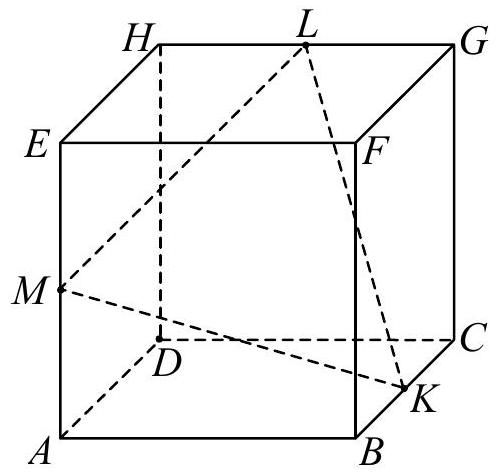
\includegraphics[max width=\textwidth, center]{2024_11_21_5b6b7ffa9006e3f448adg-18}\\

\includegraphics[max width=\textwidth, center]{2024_11_21_5b6b7ffa9006e3f448adg-18(1)}\\

\includegraphics[max width=\textwidth, center]{2024_11_21_5b6b7ffa9006e3f448adg-19(1)}

Odpowiedź:\\
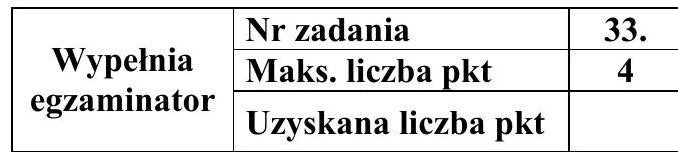
\includegraphics[max width=\textwidth, center]{2024_11_21_5b6b7ffa9006e3f448adg-19}

\section*{BRUDNOPIS}
\begin{center}
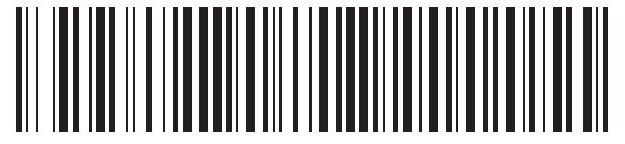
\includegraphics[max width=\textwidth]{2024_11_21_5b6b7ffa9006e3f448adg-21}
\end{center}

MMA-P1\_1P-112

WYPEŁNIA ZDAJACY

PESEL\\
\(\square\)

Miejsce na naklejkę z nr PESEL

\begin{center}
\begin{tabular}{|c|c|c|c|c|}
\hline
\begin{tabular}{l}
Nr \\
zad. \\
\end{tabular} & \multicolumn{4}{|l|}{Odpowiedzi} \\
\hline
1 & A & B & C & D \\
\hline
2 & A & B & C & D \\
\hline
3 & A & B & C & D \\
\hline
4 & A & B & C & D \\
\hline
5 & A & B & C & D \\
\hline
6 & A & B & C & D \\
\hline
7 & A & B & C & D \\
\hline
8 & A & B & C & D \\
\hline
9 & A & B & C & D \\
\hline
10 & A & B & C & D \\
\hline
11 & A & B & C & D \\
\hline
12 & A & B & C & D \\
\hline
13 & A & B & C & D \\
\hline
14 & A & B & C & D \\
\hline
15 & A & B & C & D \\
\hline
16 & A & B & C & D \\
\hline
17 & A & B & C & D \\
\hline
18 & A & B & C & D \\
\hline
19 & A & B & C & D \\
\hline
20 & A & B & C & D \\
\hline
21 & A & B & C & D \\
\hline
22 & A & B & C & D \\
\hline
23 & A & B & C & D \\
\hline
\end{tabular}
\end{center}

WYPEŁNIA EGZAMINATOR

\begin{center}
\begin{tabular}{|r|c|c|c|c|c|c|}
\hline
Nr & \multicolumn{6}{|c|}{Punkty} \\
\hline
zad. & \(\mathbf{0}\) & \(\mathbf{1}\) & \(\mathbf{2}\) & \(\mathbf{3}\) & \(\mathbf{4}\) & \(\mathbf{5}\) \\
\hline
\(\mathbf{2 4}\) & \(\square\) & \(\square\) & \(\square\) &  &  &  \\
\hline
\(\mathbf{2 5}\) & \(\square\) & \(\square\) & \(\square\) &  &  &  \\
\hline
\(\mathbf{2 6}\) & \(\square\) & \(\square\) & \(\square\) &  &  &  \\
\hline
\(\mathbf{2 7}\) & \(\square\) & \(\square\) & \(\square\) &  &  &  \\
\hline
\(\mathbf{2 8}\) & \(\square\) & \(\square\) & \(\square\) &  &  &  \\
\hline
\(\mathbf{2 9}\) & \(\square\) & \(\square\) & \(\square\) &  &  &  \\
\hline
\(\mathbf{3 0}\) & \(\square\) & \(\square\) & \(\square\) &  &  &  \\
\hline
\(\mathbf{3 1}\) & \(\square\) & \(\square\) & \(\square\) & \(\square\) & \(\square\) &  \\
\hline
\(\mathbf{3 2}\) & \(\square\) & \(\square\) & \(\square\) & \(\square\) & \(\square\) & \(\square\) \\
\hline
\(\mathbf{3 3}\) & \(\square\) & \(\square\) & \(\square\) & \(\square\) & \(\square\) &  \\
\hline
\end{tabular}
\end{center}

\begin{center}
\begin{tabular}{|c|c|c|c|c|c|c|c|c|c|c|c|c|c|c|c|c|c|c|}
\hline
\multicolumn{19}{|l|}{\multirow[t]{3}{*}{\begin{tabular}{l}
SUMA \\
PUNKTÓW \\
D \(\square\) \(\square\) \(\square\) \(\square\) \(\square\) \(\square\) \(\square\) \(\square\) \(\square\) \(\square\) \( \begin{array}{llll} 0 & 1 & 2 \end{array} \) \\
4 \\
5 \\
67 \\
8 \\
9 \\
J \(\square\) \(\square \square\) \(\square\) \(\square\) \(\square\) \(\square\) \(\qquad\) \(\qquad\) \(\square\) \(\square\) \(\qquad\) \(\square\) \(\qquad\) \(\qquad\) \(\qquad\) \(\square\) - 1 \(\qquad\) \(\qquad\) 89 \(\qquad\) \\
\end{tabular}}} \\
\hline
 &  &  &  &  &  &  &  &  &  &  &  &  &  &  &  &  &  &  \\
\hline
 &  &  &  &  &  &  &  &  &  &  &  &  &  &  &  &  &  &  \\
\hline
\end{tabular}
\end{center}

\begin{center}
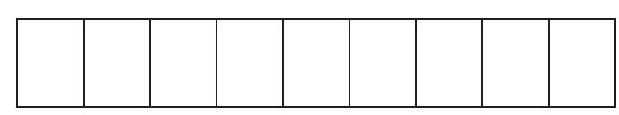
\includegraphics[max width=\textwidth]{2024_11_21_5b6b7ffa9006e3f448adg-22(1)}
\end{center}

\section*{KOD EGZAMINATORA}
Czytelny podpis egzaminatora\\
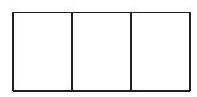
\includegraphics[max width=\textwidth, center]{2024_11_21_5b6b7ffa9006e3f448adg-22}

KOD ZDAJĄCEGO


\end{document}